%
% File - ch1.tex
%
%
% Description:
% This file should contain the first real chapter or section of your
% thesis.
%
%
The experimental results show that in many cases the GPU out-performs the CPU as
expected.  

\section{Results}
The performance is compared in terms of the number of polygons that can be queried per second. The number of polygons queried per second is measured for a wide range of input points. As the size of  data points increase, the performance of CPU diminishes at a faster rate than the GPU. In the case of GPUs, as the size of input increases, performance is affected as the amount of work done per thread increases and also the overhead of memory transfer of large amount of data between CPU and GPU increases.  But once the quadtree is transferred to the GPU, any number of polygons can be queried using iterative BFS traversal method described above.

Figure~\ref{fig:CPU_GPU_SmallPoly3}, Figure~\ref{fig:CPU_GPU_MediumPoly3} and Figure~\ref{fig:CPU_GPU_LargePoly3} show that the CPU-GPU approach gives a performance improvement 
by a factor of 3.2 for small datasets and a performance improvement by a factor of 449 for very large datasets in the case of small polygons, a performance improvement by a factor of 4 for small datasets and a performance improvement by a factor of 594 for very large datasets in the case of medium sized polygons and a performance improvement by a factor of 3.6 for small datasets and a performance improvement by a factor of 591 for very large datasets in the case of large sized polygons respectively.

\begin{figure}[H]
\centering
\vspace{0.5in}
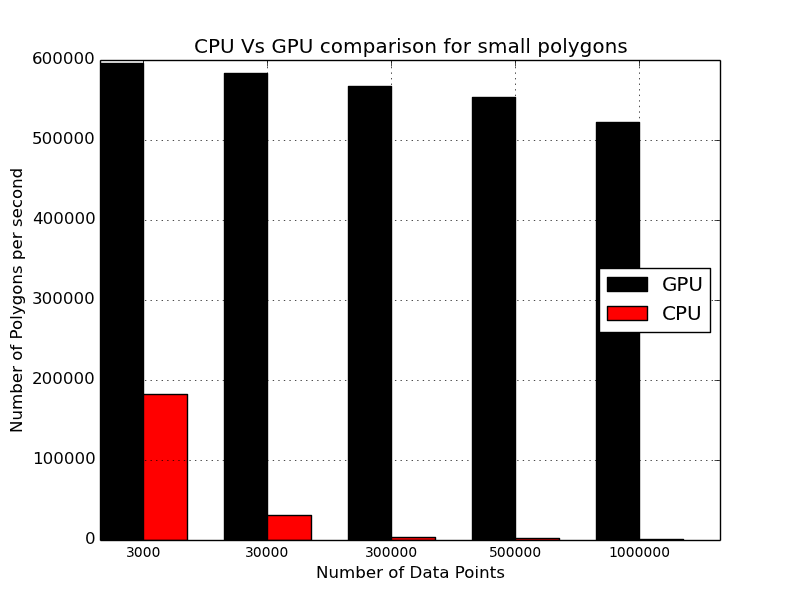
\includegraphics[scale=0.5]{Images/CPU_GPU_SmallPoly3}
\vspace{0.5in}
\caption{Performance Comparison between CPU and GPU for Small Polygons.}
\label{fig:CPU_GPU_SmallPoly3}
\end{figure}

\begin{figure}[H]
\centering
\vspace{0.5in}
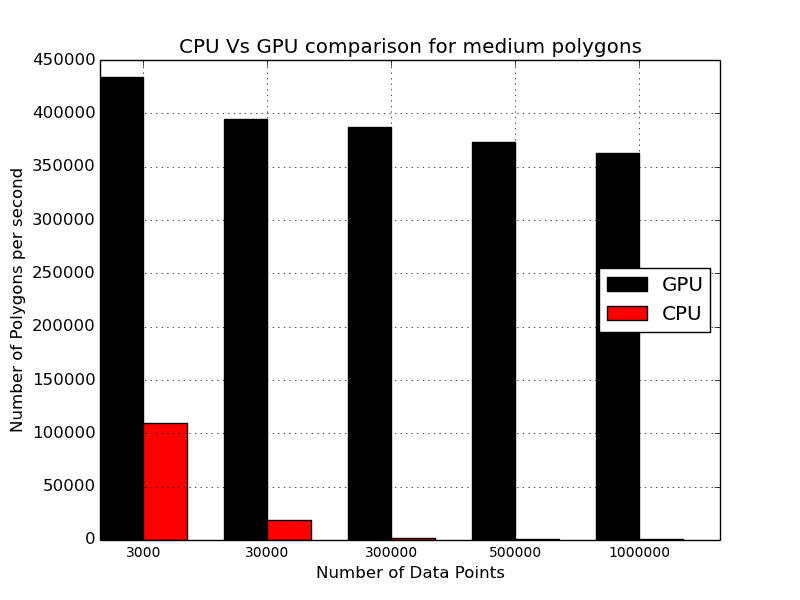
\includegraphics[scale=0.5]{Images/CPU_GPU_MediumPoly3}
\vspace{0.5in}
\caption{Performance Comparison between CPU and GPU for Medium Polygons.}
\label{fig:CPU_GPU_MediumPoly3}
\end{figure}

\begin{figure}[H]
\centering
\vspace{0.5in}
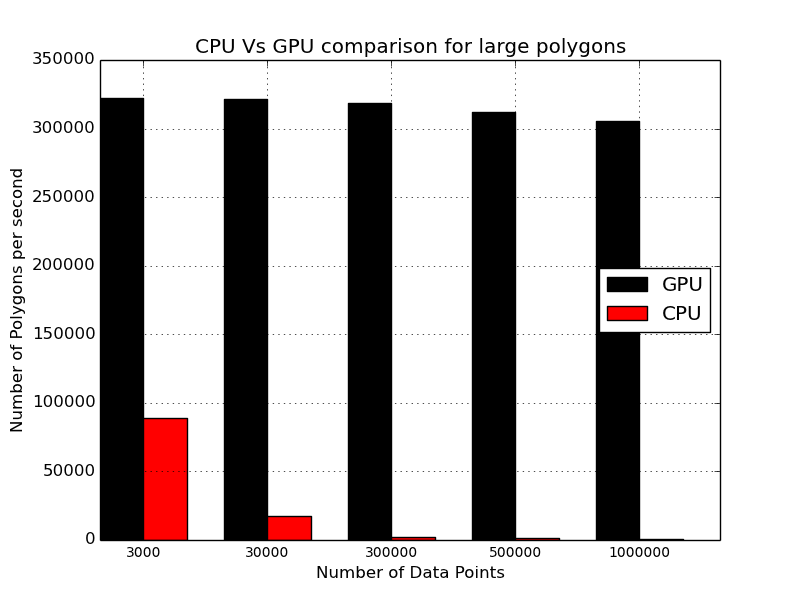
\includegraphics[scale=0.5]{Images/CPU_GPU_LargePoly3}
\vspace{0.5in}
\caption{Performance Comparison between CPU and GPU for Large Polygons.}
\label{fig:CPU_GPU_LargePoly3}
\end{figure}

The CPU performance diminishes at a faster rate than the GPU mainly because of the quadtree structure and the memory hierarchy. Since the tree is a pointer based structure, there is a cache miss every time a node is accessed. At the leaf node, the points are stored in a linked list, where each node in the list contains a pre-determined number of points and there is a cache miss every time a new buffer in the list is accessed. Therefore cache miss penalties are higher for larger datasets.

In the case of GPUs, the point buffers are sequentially stored in memory through memory preallocation. Though there is a penalty when a node is accessed, cache miss penalties are not encountered while reading data points from a node. And also, in the GPU implementation, the traversal is accelerated by starting the BFS at level 3 of the quadtree.

The Figure~\ref{fig:Different_Sized_Polygon_GPU4} shows the execution time of different polygon sizes on GPU. Similar to CPU, the GPU performs better on smaller polygons compared to the larger polygons.
In this case, the smaller polygons occupy 10 to 20 percent of the region  and the larger polygons occupy 70 to 90 percent of the region. Once the leaf nodes are reached, the number of nodes that need to be taken into account to compute points are very less  but for a large polygon which could contain a maximum of 64 nodes for a level 4 quadtree, points within all these 64 nodes need to be taken into account.

\begin{figure}[H]
\centering
\vspace{0.5in}
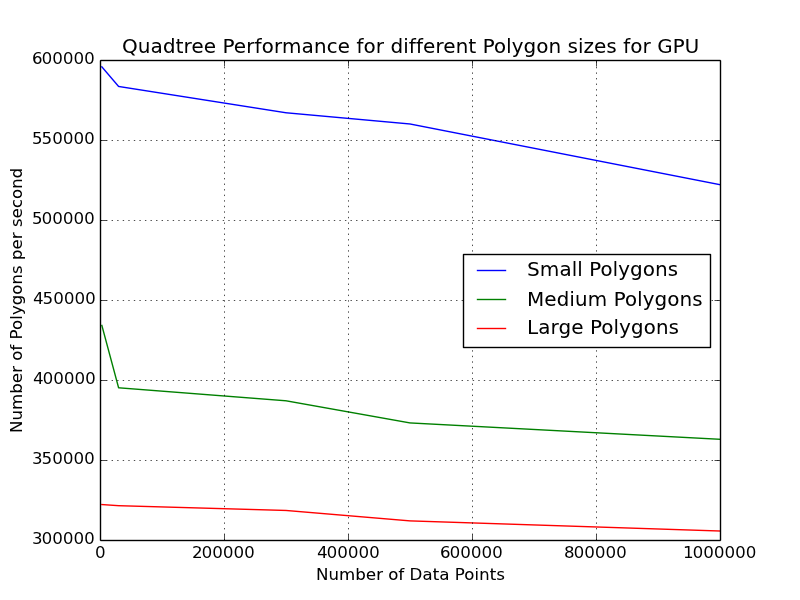
\includegraphics[scale=0.5]{Images/Different_Sized_Polygon_GPU4}
\vspace{0.5in}
\caption{Performance Comparison for Different Sized Polygons using GPU.}
\label{fig:Different_Sized_Polygon_GPU4}
\end{figure}

The performance is determined by the number of partial nodes a polygon contains because for partial nodes, each point inside a node needs to be checked against a polygon boundary whereas in the case of completely overlapping nodes only the range of points a node contains is stored.
The Figure~\ref{fig:LToMCmplxMedP} shows the execution time of individual medium sized polygons with a data input size of 3000. The polygons are ranked based on the number of partial nodes it contains and its execution time is measured. As the number of partial nodes increase, the execution time per polygon increases.
The number of polygons calculated per second is the average of the output of all these individual polygons.

\begin{figure}[H]
\centering
\vspace{0.5in}
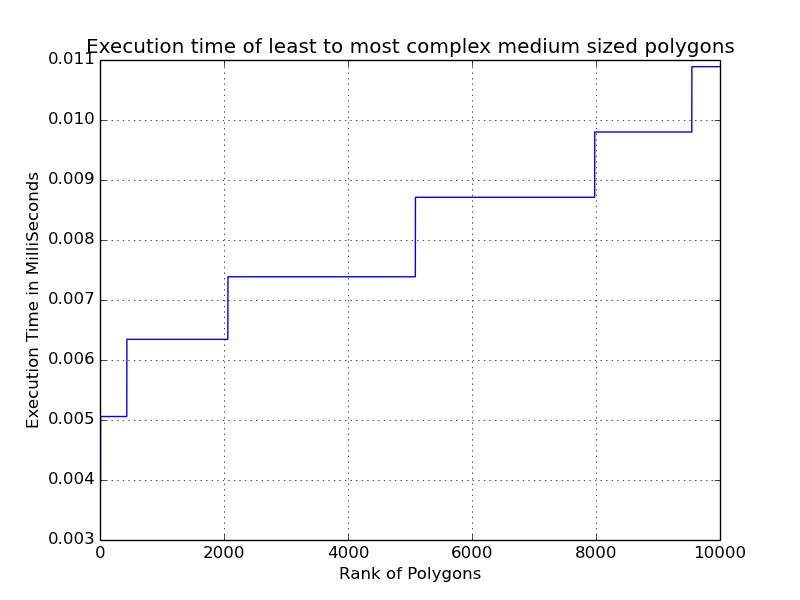
\includegraphics[scale=0.5]{Images/LToMCmplxMedP}
\vspace{0.5in}
\caption{Execution Time of Least to Most Complex Medium Sized Polygons.}
\label{fig:LToMCmplxMedP}
\end{figure}

Figure~\ref{fig:SpeedUp} shows the performance comparison between CPU and GPU measured for different sizes of polygons. The significant speed up on GPU is due to the memory coalesced access and due to accelerating the traversal by starting the BFS from level 3. In this case, the algorithm traverses one level down the tree to quickly find the set of nodes that satisfy the query, 

The maximum performance gain is achieved for the medium polygons which are more computationally intensive than small polygons. Very less number of threads are active for small polygons and this does not take advantage of the throughput oriented nature of the GPU. The work on medium sized polygons is optimum for the GPU as the performance decreases a little for larger polygons. The performance is mainly determined by the number of partial nodes a polygon contains. In the case of CPU, all the partial nodes in a polygon are processed sequentially but in the case of GPU, 32 partial nodes within a polygon are computed in parallel with 48 (Total number of SMX x (CUDA cores per SMX / number of polygons per warp))~\cite{nvidia:12:gtx680tech} polygons being computed simultaneously.

\begin{figure}[H]
\centering
\vspace{0.5in}
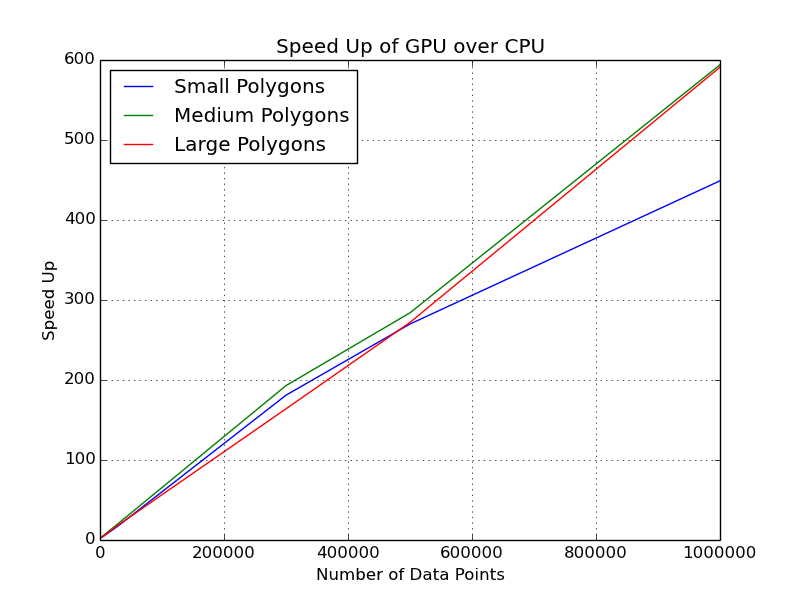
\includegraphics[scale=0.5]{Images/SpeedUp}
\vspace{0.5in}
\caption{Speed Up of GPU over CPU.}
\label{fig:SpeedUp}
\end{figure}


